%%%%%%%%%%%%%%%%%%%%%%%%%%%%%%%%%%%%%%%%%%%%%%%%%%%%%%%%%%%%%%%
%%%%%%%%%%%%%%%%%%%%%%%%%%%%%%%%%%%%%%%%%%%%%%%%%%%%%%%%%%%%%%%
%%%%%%%
%%%%%%% The Contagion of Drug Violence: 
%%%%%%% Spatio-temporal Dynamics of the Mexican War on Drugs
%%%%%%%
%%%%%%% Compiled in: www.sharelatex.com
%%%%%%%
%%%%%%%%%%%%%%%%%%%%%%%%%%%%%%%%%%%%%%%%%%%%%%%%%%%%%%%%%%%%%%%
%%%%%%%%%%%%%%%%%%%%%%%%%%%%%%%%%%%%%%%%%%%%%%%%%%%%%%%%%%%%%%%

\documentclass[12pt,letterpaper]{article}
\usepackage[utf8]{inputenc}
\usepackage[T1]{fontenc}
\usepackage[margin=2.5cm]{geometry}
\usepackage{amsmath}

%% Uncomment to send footnotes as endnotes
\usepackage{endnotes}                       % http://ctan.org/pkg/endnotes
\let\footnote\endnote
\def\footnotetext{\endnotetext[\number\numexpr\value{endnote}+1]}
\let\footnotemark\endnotemark


\usepackage{array}                          %For centering justified text in tables%
\usepackage{setspace}                       % To shrink space between lines %
\doublespacing                              % Uncomment for single spacing%

\usepackage{latexsym}
\usepackage{longtable}                      % For tables across multiple pages
\usepackage{multirow}                       % For tables with a cell covering multiple rows
\usepackage{lscape}                         % Horizontal page %
\usepackage{chngcntr}
\usepackage{caption}
\usepackage{float}                          % For tables and graphs  %
\usepackage[capposition=top]{floatrow}      %For adding a note below a figure%
\usepackage{booktabs,caption,fixltx2e}      %For adding a note below a figure%
\usepackage[flushleft]{threeparttable}      %For adding a note below a figure%
\usepackage{subfigure}
\usepackage[demo]{graphicx}
\usepackage{caption}
\usepackage{subcaption}


\usepackage{chicago}  
\usepackage{natbib}              % Bibliography %
\bibpunct[; ]{(}{)}{,}{a}{}{;}   % Uncomment this to eliminate coma in citations%
\setlength{\bibsep}{1.9 pt}      %To reduce space between lines in the bilbiography%


\usepackage[all,defaultlines]{nowidow}      % Prevents widows and orphans %



\newcommand{\N}{\mathrm{N}}

\usepackage{authblk}        % Author affiliation %

%%%%%%%%%%%%%%%%%%%%%%%%%%%%%%%%%%%%%%%%%%%%%%%%%%%%%%%%%%%%%%%
%%%%%%%%%%%%%%%%%%%%%%%%%%%%%%%%%%%%%%%%%%%%%%%%%%%%%%%%%%%%%%%

\title{The Contagion of Drug Violence: Spatio-temporal Dynamics of the Mexican War on Drugs}

\author{Javier Osorio} % Comment for making paper anonymous %

\affil{John Jay College of Criminal Justice\\ City University of New York}

%\footnotemark{Assistant Professor, John Jay College of Criminal Justice, City University of New York. This research was made possible thanks to the support of the National Science Foundation; the Social Science Research Council -- Open Society Foundations; the United States Institute of Peace; the Kellogg Institute at the University of Notre Dame; the Harry Frank Guggenheim Foundation; the Program on Order, Conflict and Violence at Yale University; and the Mario Einaudi Center for International Studies at Cornell University. Contact: josorio@jjay.cuny.edu}



\date{January, 2015}





%%%%%%%%%%%%%%%%%%%%%%%%%%%%%%%%%%%%%%%%%%%%%%%%%%%%%%%%%%%%%%%
%%%%%%%%%%%%%%%%%%%%%%%%%%%%%%%%%%%%%%%%%%%%%%%%%%%%%%%%%%%%%%%
\begin{document}

\maketitle


%%%%%%%%%%%%%%%%%%%%%%%%%%%%%%%%%%%%%%%%%
%\mbox{}\\
\mbox{}\\
\begin{spacing}{1.0}
\begin{abstract}
\noindent Why are some territories ravaged by intense levels of criminal violence while others are relatively peaceful? This research contributes to an understanding of the escalation and diffusion of drug violence in Mexico from 2000 to 2010 by formalizing the interactions between the state and organized criminals and by relying on a large database of event data containing more than 1.6 million observations. Results based on spatial econometrics provide evidence of the spatial diffusion of violence. In congruence with the theoretical expectations, the results show that the disruptive effect of law enforcement is an important catalyst for the intensification of violence between criminal organizations, especially when deployed in areas hosting a high concentration of criminal groups. This relationship holds for a broad menu of violent and non-violent law enforcement tactics. The analysis also reveals that other broadly held factors (international, geographic, and socioeconomic characteristics) have a modest effect on the dynamics of drug-related violence. \\ \\
\mbox{}\\
%\mbox{}\\
\emph{Keywords:} Drug violence, Mexico, diffusion, event data.  \\ \\
\emph{Word count:} 10,550 words \\ \\
\end{abstract}
\end{spacing}


\newpage

%%%%%%%%%%%%%%%%%%%%%%%%%%%%%%%%%%%%%%%%%
\section*{Introduction}

During the past few years Mexico has experienced an unprecedented increase in drug-related violence. This wave of violence is puzzling because drug trafficking organizations (DTOs) have existed in Mexico for decades without engaging in systematic confrontations against the state or rival criminal groups on such a scale. Following early debates about whether or not government efforts to fight crime triggered the escalation of criminal violence,\footnote{See \citet{Guerrero2011}, \citet{Poire2011}, \citet{Shirk2010}, \citet{Rios2011}, \citet{Astorga2005}, \citet{Donnelly2010} and \citet{Cornelius2007}.} the emerging quantitative literature on the Mexican war on drugs has provided compelling evidence indicating that government crackdowns substantially contributed to the escalation of violence between DTOs \citep{Calderon2012,Dell2011,Osorio2013}. However, the spatial diffusion patterns of drug-related violence have remained largely underexplored. Why are some regions of the country ravaged by intense levels of criminal violence while others remain relatively peaceful? What are the structural and dynamic determinants of the spatial contagion of conflict?

As indicated by \citeauthor*{Shirkthisissue} (\emph{this issue}), recent studies on the Mexican war on drugs have focused on analyzing either the political determinants of violence \citep{Snyder2009a,DuranMartinez2012,Rios2012a,Osorio2013,Dell2011} or the effect of law enforcement on the escalation of conflict \citep{Guerrero2011,Calderon2012,Dell2011}. Other authors point to the availability of weapons and international drug supply shortages as possible causes \citep{Dube2013,Castillo2014}. Although researchers have identified patterns of spatial dispersion of drug violence in Mexico \citep{Guerrero2011a,Molzahn2013}, our understanding of the specific mechanisms of contagion still is in an early stage \citep{Dell2011,Ingram2014}. Among the explanations of diffusion, Dell's \citeyearpar{Dell2011} study argues that law enforcement along drug-transit routes generates a spillover of violence to alternate routes as DTOs relocate to other territories. This approach offers a \emph{centrifugal} explanation of conflict in which DTOs \emph{divert} their areas of operation as they try to avoid law enforcement. 

In contrast to the centrifugal approach, the explanation advanced in this research offers a \emph{centripetal} account of drug violence. The argument claims that increasing law enforcement undermines the capabilities of local criminal groups to defend their territories, thus \emph{attracting} efforts of territorial conquest from neighboring criminal organizations. Based on a formal model, the theoretical explanation claims that law enforcement disrupts the relative military balance among DTOs by weakening a criminal organization and indirectly improving the position of its rivals. This improvement might motivate an invasion from a competing DTO in an effort to capture the territory of the weakened DTO, thus setting in motion a turf war over valuable territories. The disruptive effect of law enforcement is magnified when deployed in areas with a high density of criminal organizations.    

The empirical evidence comes from a large database of weekly event data from 2000 to 2010 at the municipal level comprising more than 1.6 million observations. The database provides detailed information on the intensity of inter-cartel violence and a broad menu of violent and non-violent law enforcement tactics employed by the state to fight crime. Based on the use of spatial econometrics, the results provide  evidence for the diffusion of violence from neighboring areas. In congruence with the centripetal account, the statistical assessment reveals that the escalation and diffusion of violence between DTOs are primarily explained by the disruptive effect of law enforcement in areas containing a larger number of criminal groups. When considered individually or as interaction terms, both the intensification of law enforcement and the increasing number of DTOs are positively associated with the severity of violence between criminal organizations. In contrast, depending on the type of law enforcement tactic used by the authorities, the statistical assessment finds contradictory evidence or weak support for the centrifugal explanation of violence.

The statistical analysis also suggests that drug-valuable territories play a marginal role in explaining violence. In addition, the results question other major arguments emphasizing the availability of weapons, shocks in the international supply of drugs, corruption, poverty, and education as central factors accounting for violence among criminal organizations. In general, the empirical assessment shows that the rapidly changing interactions between state security forces and criminal groups, as well as exposure to violence from neighboring areas, play a larger role in explaining inter-cartel violence than the modest contribution of structural factors and contextual characteristics.

The article is organized as follows. The following section presents the formal model illustrating how law enforcement triggers territorial competition between criminal groups and derives a set of empirical implications. The next section describes the data on drug violence and other covariates. Next, the spatial descriptive statistics identify the upsurge and intensity of hot spots of violence. This is followed by an empirical assessment with a discussion of the specification of the spatial econometric model and a report of the statistical results. The conclusions are presented in the final section.  





%%%%%%%%%%%%%%%%%%%%%%%%%%%%%%%%%%%%%%%%%
\section*{A theory of criminal competition}

Following research on territorial competition \citep{Skaperdas2002,Carter2010,Osorio2013}, this work advances a model of multi-polar competition among criminals. The model uses a basic contest success function \citep{Tullock1980,JiaSkaperdasVaidya2009} to explain how law enforcement disrupts the military equilibrium between drug cartels and triggers a wave of territorial competition among them. Consider two adjacent territories $1$ and $2$ of equal strategic value $\tau > 0$. For now, let there be four criminal organizations $P={a,b,c,d}$. Assume that each DTO is a unitary actor.\footnote{In this sense, the model does not directly analyze intra-cartel violence in which factions fight over the control of the organization. If a DTO splits and its different factions fight each other --as happened with the Golfo Cartel vs. Los Zetas-- the model considers them as two distinct DTOs.} Each territory is populated by two criminal groups such that DTOs $a$ and $b$ are located within the boundaries of Territory $1$ and DTOs $c$ and $d$ in Territory $2$. Criminals use their military strength to extract rents from a share of the territory they can control, such that $M_{ij}\tau$. The relative military strength of each pair of players is determined by a contest success function $M_{ij} \in [0,1]$ expressing the probability of player $i$ winning a fight against player $j$. $M_{ij}$ depends on the relative military strength of each player with respect to its neighbor;
\begin{equation}
M_{ij} = \frac{w_{i}}{w{i}+w{j}},
\label{eq:contest}
\end{equation}
where $w_{i}>1$ represents military resources such as the \emph{sicarios} (hitmen) that DTO $i$ employs as fighters, $w_{j}>1$ are the hitmen used by player $j$, and $w_{i}+w{j}$ represents the total hitmen allocated by both parties. The contest success functions pair $i$ and $j$ are constrained to add to 1; that is, $M_{ij}+M_{ji}=1$. This implies that $M_{ij}$ and $M_{ji}$ are reciprocal;  $M_{ij}= 1-M_{ji}$. 

Assume a status quo situation in which all players have equal military capabilities, $M_{ab}=M_{ba}=M_{cd}=M_{dc}=1/2$, which allows each to control an equal share of their respective areas. This implies that the four DTOs are equally spaced along the territories as illustrated in Panel (a) in Figure \ref{fig:territorial_competition}. Territory $1$ is represented by the solid line and Territory $2$ as a dashed line in Figure \ref{fig:territorial_competition}. Assume that each DTO controls the portion of the territory located to the left of its position and extending to the right edge of its neighbor's position. Because of geography and transportation costs, assume that DTOs can only wage war against their contiguous neighbors and expand their domains only to their immediate vicinity. For simplicity, consider first the effect of law enforcement on the interaction between DTOs $a$ and $b$ in Territory $1$. Let government authorities enforce the law against DTO $b$, thus undermining its military capabilities by a factor of $\varepsilon_{b} \le M_{ba}$, where $\varepsilon_{b}$ represents the amount of damage inflicted by law enforcement on DTO $b$ such that $M^{\prime}_{ba}=M_{ba}-\varepsilon_{b}$. This shows that law enforcement weakens DTO $b$, thus leading to $M^{\prime}_{ba}<M_{ba}$.

\begin{center}
   [Insert Figure~\ref{fig:territorial_competition} about here]
\end{center}


According to this model, state action has a non-neutral effect on the relative military balance among criminal groups. By enforcing the law against DTO $b$, the state indirectly improves the relative military position of DTO $a$, which now faces a weaker rival as indicated by $M_{ab}+\varepsilon_{b}>M^{\prime}_{ba}$. This improved relative position might motivate $a$ to attack $b$ in an attempt to acquire its territory. The invasion from DTO $a$ further diminishes $b$'s military capabilities by $\gamma_{ab}$, such that $M^{\prime \prime}_{ba}=M^{\prime}_{ba}-\gamma_{ab}$, where $\gamma_{ab}<=M^{\prime}_{ba}$ represents the amount of damage caused by $a$ on $b$. After the invasion, player $b$'s relative military position is reduced to $M^{\prime \prime}_{ba}$, where $M^{\prime \prime}_{ba}<M^{\prime}_{ba}<M_{ba}$. 

Now let DTO $b$ retaliate against the invader $a$. It manages to recover part of the lost territory by $\sigma_{b}$, such that  $M^{\prime \prime \prime}_{ba}=M^{\prime \prime}_{ba}+\sigma_{ba}$, where $\sigma_{ba}\le 1$ represents the ability of DTO $b$ to recover from invasion by $a$. After fighting back against the trespasser, the relative military position of DTO $b$ with respect to DTO $a$ is improved to $M^{\prime \prime \prime}_{ba}$, which for illustrative purposes is assumed to be  $M_{ba} < M^{\prime}_{ba} < M^{\prime \prime \prime}_{ba}<M^{\prime \prime}_{ba}$. This indicates that after the violent interactions between DTOs $a$ and $b$ caused by law enforcement, the relative military position of $b$ is weaker than at the status quo.  

As indicated in Panel (b) in Figure \ref{fig:territorial_competition}, DTO $b$ is now in a vulnerable situation with respect to DTO $c$ in the neighboring territory. After being the recipient of law enforcement and attacks by criminal group $a$, DTO $b$ might have difficulty keeping neighboring rival $c$ at bay. Based on the rationale discussed above, DTO $c$ might launch an invasion against a weak DTO $b$ in Territory 1. This attack might further reduce $b$'s military capabilities from $M_{bc}$ to $M^{\prime}_{bc}=M_{bc}-\gamma_{cb}$. As indicated above, DTO $b$ might fight back against the invader $c$ and recover part of the lost territory up to $M^{\prime\prime}_{bc}=M^{\prime}_{bc}+\sigma_{bc}$. At the end of the violent interaction between these two criminal groups, DTO $b$ is weaker than before and DTO $c$ has not only gained strength but also managed to secure a fraction of Territory $1$.  

The model also identifies conditions favoring the spillover of violence. The conquest of new territories by DTO $c$ further improves its relative military position with respect to a rival criminal group $d$ based in Territory $2$, as illustrated by Panel (c) in Figure \ref{fig:territorial_competition}. By the same token, now that $c$ finds a relatively weaker rival, it might launch an invasion against DTO $d$ in order to control a fraction of the territory up to $M^{\prime}_{cd}$. Incursions into $d$'s territory might generate a reaction to repel the invader and recover part of the lost territory, which would locate the new military balance at $M^{\prime\prime}_{cd}$. 

This simple model illustrates how state actions disrupt the relative military balance among rival criminal groups. Law enforcement is not only likely to unleash violent competition among DTOs coexisting within the same region, but may also motivate invasion by criminals from bordering territories and even the diffusion of violence to neighboring areas.   

Based on this intuition, now consider a general contest success function for a number $\N$ of DTOs, where $\N >1$. Assume that DTO $i$ receives the benefits from a territory of certain value ($\tau$) that it can control given its military capabilities relative to those of its neighbors. Consider that all DTOs have the same number of warriors, such that $w_{i}=w_{j}$. In addition, hiring \emph{sicarios} represents a cost of $\beta>0$. Also assume that geographical factors such as distance, represented by $\theta>0$, further increase the costs of fighting as it takes a larger effort to wage war in distant territories. This leads to the following payoff;
\begin{equation}
\frac{w_{i}}{w_{i}+\sum^{N}_{j\neq i}(w_{j} - \varepsilon_{j} -\gamma_{\sim j j} +\sigma_{j \sim j})}(\tau)-\theta\beta w_{i},
\label{eq:rent}
\end{equation}
where $\sum^{N}_{j\neq i}(w_{j} - \varepsilon_{j} -\gamma_{\sim j j} +\sigma_{j \sim j})$ represents the total military strength of $i$'s rivals, such that $j=1, 2, \dots N$, while considering the effect of enforcement, invasion and retaliation. From equation \eqref{eq:rent}, it is clear that as $\N$ increases, the rents for DTO $i$ decrease. This means that areas with a higher density of criminal organizations yield lower net benefits for each criminal group in the area. As a result, DTO $i$ benefits if the strength of any of its rivals or the total number of rivals is reduced -- which may be caused by the use of law enforcement. This can be illustrated with comparative statics by introducing state crackdowns on rival DTOs ($\varepsilon_{j}$) on the right side of equation \eqref{eq:rent_enforcement}:
\begin{equation}
\frac{w_{i}}{w_{i}+\sum^{N}_{j\neq i}w_{j}}(\tau)-\theta\beta w_{i} < \frac{w_{1}}{w_{i}+\sum^{N}_{j\neq i}(w_{j}-\varepsilon_{j})}(\tau)-\theta\beta w_{i}.
\label{eq:rent_enforcement}
\end{equation}

The same logic applies if we substitute for law enforcement the damage caused by territorial invasion ($\gamma_{\sim j j}$) of competitor $ \sim j$ against a rival DTO $j$. Assuming no retaliation against the invasion ($\sigma_{j\sim j}=0$) leads to the following comparative statics:
\begin{equation}
\frac{w_{i}}{w_{i}+\sum^{N}_{j\neq i}w_{j}}(\tau)-\theta\beta w_{i} < \frac{w_{1}}{w_{i}+\sum^{N}_{j\neq i}(w_{j}-\gamma_{\sim jj})}(\tau)-\theta\beta w_{i}.
\label{eq:rent_invasion}
\end{equation}

In this case, DTO $i$ improves its military position with respect to criminal group $j$ if the latter is invaded by a third rival $\sim j$. The right side of equation \eqref{eq:rent_invasion} also elucidates the conditions favorable for the diffusion of violence. Under generalized competition, DTO $i$ might launch an invasion against its rivals if the benefits associated with the probability of winning the battle are larger than the costs of fighting; that is,
\begin{equation}
\frac{w_{1}}{w_{i}+\sum^{N}_{j\neq i}(w_{j}-\gamma_{\sim j})}(\tau)>\theta\beta w_{i}.
\label{eq:invasion_condition}
\end{equation}

As discussed above, it can be assumed that $\frac{w_{i}}{w_{i}+\Sigma^{N}_{j\neq i}w_{j}}$ represents the probability of DTO $i$ winning a battle against all other criminal groups operating in the area. The Nash equilibrium for the optimal allocation of military effort by DTO $i$ is represented by
\begin{equation}
w^{*}=\frac{(\N-1)\tau}{\N^{2}(w_{j} - \varepsilon_{j} -\gamma_{\sim j j} +\sigma_{j \sim j})\theta\beta}.   
\label{eq:equilibrium}
\end{equation}

This shows that augmenting the number of rival criminal organizations intensifies competition and motivates DTO $i$ to increase its military effort to maintain the same level of rents. Thus, a high density of criminal groups operating in an area is associated with more violence between them. Equation \eqref{eq:equilibrium} also provides insights about the strategic importance of some locations. In highly valuable areas, criminal organizations have more incentives to increase their military effort toward either capturing or protecting the territory. This suggests that violence has a tendency to concentrate around highly valuable or strategic locations. In addition, low values of parameter $\theta$ suggest that geographic conditions such as proximity or plain terrain might reduce the overall costs of fighting and facilitate invasion of criminal groups against their neighboring groups.

Based on the dynamics captured by the model, it is possible to derive the following testable implications:
\begin{spacing}{0.9}
\begin{description}
\item [] $H_{1}$: Increasing violence between DTOs in a territory is positively associated with violence between DTOs in neighboring areas. 
\item [] $H_{2}$: Increasing law enforcement is positively associated with violence between DTOs. 
\item [] $H_{3}$: A greater number of DTOs is positively associated with violence between DTOs. 
\item [] $H_{4}$: Increasing law enforcement in areas with a high density of criminal organizations is  associated with more violence between DTOs than enforcement in areas with a lower density.
\end{description}
\end{spacing}

\noindent In this way, hypotheses $H_{2}$, $H_{3}$  and  $H_{4}$ elucidate the mechanisms of conflict operating within a location, whereas hypothesis $H_{1}$ pertains to the contagion of violence to other locations.



%%%%%%%%%%%%%%%%%%%%%%%%%%%%%%%%%%%%%%%%%
\section*{Event data on drug violence}

The empirical evidence comes from Organized Criminal Violence Event Data (OCVED), a large database containing events of drug-related violence in Mexico at the municipal level from 2000 to 2010. Following efforts using automated textual annotation for studying conflict \citep{Leetaru2013}, OCVED relies on \emph{Eventus ID}, a novel software for coding event data from news reports written in Spanish \citep{Osorio2014}. Using a similar algorithm to that implemented by \citet{Schrodt2009} in \textsc{Tabari}, Eventus ID identifies three key components of event data: the perpetrator of an action, known as the \emph{source}; the specific \emph{action} being conducted; and the \emph{target} of the action. For example, in the sentence ``a group of hitmen killed a police officer,'' Eventus ID codes ``a group of hitmen'' as the source, the verb ``killed'' as the action  and ``police officer'' as the target. The software also records the date and geographic location when such information is available in the report. Based on the source-action-target structure, OCVED comprises different types of events of violence between criminal groups, as well as a variety of law enforcement tactics directed against DTOs. In this way, the data provides detailed information on who did what to whom, when, and where in the Mexican war on drugs. OCVED contains event data on a daily basis. However, the statistical assessment required aggregating data at the week level to ease the computational demands of conducting spatial econometric analysis.    

OCVED gathers information from 105 different sources written in Spanish, including federal and local government agencies, as well as national and local newspapers\footnote{The Appendix reports the detailed list of information sources.} from 2000 to 2010. The variety of information sources mitigates concerns of bias in media-based databases \citep{Davenport2002,Davenport2009a}. To reduce the risk of redundant inclusions caused by multiple sources reporting prominent events, duplicates were identified and excluded from the database using standard statistical procedures. In addition, the extent of media freedom and independence in the democratic era of the Mexican political system reduces concerns of bias from the use of government sources \citep{Lawson2002}. Notwithstanding their methodological differences, the comparison of OCVED and other homicide databases indicates a high level of correlation, ranging from r=0.69 to r=0.73, thus providing a consistent description of the trends of violence (\citeauthor*{Shirkthisissue} \emph{this issue}).\footnote{The Appendix presents the correlation assessment between OCVED and other databases.} Nevertheless, despite careful measurement efforts, OCVED may still have limitations in grasping a phenomenon that is inherently difficult to measure \citep{Andreas2010,Seybolt2013}.

As originally implemented by \citet{Osorio2013b}, the event coding protocol consists of four stages. First, a team of trained coders ran a systematic query in Infolatina, a large repository of newspapers, which yielded hundreds of thousands of possibly relevant reports. Second, based on the search output, coders followed strict coding rules\footnote{News reports were included if they mentioned the traditional \emph{modus operandi} of organized criminals which includes the use of high-caliber weapons, violence perpetrated by groups of armed men, use of convoys of vehicles, multiple victims, bodies with multiple bullet wounds, bodies shot execution-style in the head, signs of torture or mutilation, or written messages left near the victims. The criteria excluded reports of ordinary crimes (e.g., robbery, burglary), actions perpetrated by insurgents, and statements or opinions about drug violence. Reports were thus considered only if they mentioned facts, not discussions about those episodes.} to identify news reports of violence committed either by criminal groups or by government authorities conducting law enforcement activities. This labor intensive stage generated a selection of 41,838 reports. Third, the selected reports served as input text for automated event coding using Eventus ID, which generated the raw event data. The fourth stage consisted of validating, aggregating, and recoding the data, which led to several iterations of stages three and four.\footnote{The Appendix contains further details of the coding protocol and descriptive statistics of the data.} The final product was a database containing 251,167 geo-referenced events considering all municipalities of Mexico ($N$=2,456) on a daily basis from January 1\textsuperscript{st}, 2000 to December 31\textsuperscript{st}, 2010 ($T$=4,017 days), for a total ($N \times T$) of 9,865,752 municipality-days. As indicated before, the computational demands of spatial analysis in this study required reducing the number of observations by aggregating the data at the week-municipal level, for a total of 1,667,624 observations. Even at this unit of analysis, OCVED overcomes the  truncation and aggregation limitations of other databases (\citeauthor*{Shirkthisissue} \emph{this issue}). 

The dependent variable, \emph{violence between DTOs}, measures the number of violent events between criminal groups that occurred in a municipality-week. This variable is not a body-count, as it includes a variety of events such as shootings, kidnappings, homicides, confrontations, ambushes, attacks, discovery of bodies, mutilation, beheading, and torture, among other events in which the victim or the perpetrator appears to be a member of a criminal organization. The analysis also considers an array of law enforcement tactics as key independent variables. The variable \emph{violent enforcement} measures the weekly number of events in which government authorities attacked, wounded, or killed presumed organized criminals. The analysis also includes a number of non-violent enforcement tactics. The variable \emph{arrests} counts the weekly number of detentions of suspected DTO members; \emph{seizures of assets} counts the number of events in which authorities confiscated real estate or vehicles from criminals; \emph{seizures of drugs} counts the weekly number of drug interdiction events; and \emph{seizures of weapons} counts the number of episodes in which the state confiscated weapons, ammunition, or explosives.\footnote{The Appendix contains further details of the criteria used to categorize each type of event.} Despite the emphasis on disaggregation and accuracy, these variables might still under-represent the ``true'' and often unobserved amount of violence associated with the Mexican war on drugs. 

Consistent with other efforts to identify the location of DTOs \citep{Coscia2012}, Eventus ID is used for tracking the activity of criminal organizations at the municipal level.  The variable \emph{all DTOs} is a proxy measure for the total number of DTOs operating in a municipality in a given year. To provide a more nuanced analysis, this measure is disaggregated to distinguish between the numbers of \emph{main DTOs} and \emph{secondary DTOs} active in a municipality. The variable \emph{main DTOs} includes six of the most prominent drug trafficking organizations: Tijuana Cartel, Sinaloa Cartel, Juarez Cartel, Golfo Cartel, Familia Michoacana, and Los Zetas. In addition, variable \emph{secondary DTOs} comprises smaller criminal organizations, some of which emerged as spin-offs of main DTOs and others of which developed independently.\footnote{The variable secondary DTOs includes the following organizations: Cartel de Jalisco Nueva Generaci\'{o}n, La Barbie, Cartel de los Beltr\'{a}n Leyva, Cartel del Milenio, Cartel de Jalisco, Nuevo Cartel de Acapulco, La Resistencia, Los Caballeros Templarios, Cartel de Colima, Cartel de Oaxaca, La Empresa, La Mano con Ojos, Limpia Mazateca, Los Cachines and other minor criminal groups.} This qualification helps to differentiate the behavior of large consolidated DTOs from that of emerging criminal groups. 

Starting in 2006, criminal organizations underwent a process of aggressive territorial expansion. DTOs (whether major or secondary) were active in an average of 103 municipalities during any year between 2000 and 2005. But between 2006 and 2010 they expanded their territories to an average of 470 municipalities. A more detailed analysis indicates that the main cartels started a process of expansion in 2006, while smaller DTOs remained localized. In 2009, the main DTOs reached their maximum of territorial expansion, with activity in 551 municipalities (about 22.5 percent of the entire country). In the following year, their territorial activity contracted to 538 locations. In contrast, the group of emerging DTOs doubled their areas of activity, increasing from 74 municipalities in 2009 to 140 in 2010. The aggressive expansion of secondary DTOs exceeded the modest territorial contraction of the main DTOs.\footnote{The Appendix presents a graphical representation of these territorial trends.} As indicated by \citet{Arjona2011}, measures of armed group activity are imperfect indicators of their presence. Criminal organizations, just like guerrilla or paramilitary groups, may operate in an area without being detected by the authorities or the media. To reduce concerns of false negatives, the activity of a criminal organization in a location is imputed for the entire year once it is mentioned in a report. Instead of considering these measures as ``verified presence'' of criminal groups, a more cautious approach recommends seeing them as indicators of ``reported activity'' of criminal organizations.   

The operationalization of valuable territories uses different measures associated with drug-related activities.  Variable \emph{drug production} is a four-level scale rating areas where the Mexican Army identified  marijuana and poppy crops \citep{SecretariadelaDefensaNacional2011}.  Following other efforts to estimate drug consumption in Mexico \citep{Rios2012,Madrazo2012}, the variable \emph{local drug markets} is a proxy for the size of domestic drug markets and is measured as the number of cases of hospitalization caused by consumption of illegal narcotics \citep{SecretariadeSalud2012}. Variables \emph{Gulf} and \emph{Pacific} are dichotomous measures taking the value of 1 for the strip of three adjacent municipalities located along the Gulf of Mexico or the Pacific coast, which are areas favorable for the reception of drugs coming from abroad. The variable \emph{North} identifies territories favorable for international drug distribution and takes the value of 1 for the strip of three contiguous municipalities located along the Mexico--U.S.\ border. Information for these geographic variables came from INEGI  \citeyearpar{INEGI2011b}.

The variable \emph{road density} is used to assess the centrifugal account offered by \citet{Dell2011} and measures the ratio of the total length of highways contained within a municipality to the area covered by the respective municipality. This variable came from INEGI \citeyearpar{INEGI2014}. Following research on the availability of assault weapons \citep{Dube2013}, variable \emph{rifles} measures the U.S.\ production of assault rifles with data from the \citet{BureauofAlchoholTobacco2012}.  \emph{Potential cocaine production} accounts for variation in the supply of cocaine from Colombia indicated by \citet{Castillo2014} with data from the United Nations Office on Drugs and Crime, UNODC (\citeyear{UnitedNationsOfficeonDrugsandCrime2006,UnitedNationsOfficeonDrugsandCrime2013b}). Variable \emph{schooling} represents the average level of educational attainment, as employed by \citet{Ingram2014}. \emph{Cocaine price} reflects the price of a gram of pure cocaine as reported by UNODC \citeyearpar{UnitedNationsOfficeonDrugsandCrime2014} and the \citet{OfficeofNationalDrugControlPolicy2004}. The variable \emph{corruption} indicates the percentage of the state population who reported paying a bribe to avoid being arrested as reported by \citet{TransparenciaMexicana2012}. The analysis also considers the  \emph{population} size (INEGI \citeyear{INEGI2011}) and the level of \emph{poverty} \citep{CONEVAL2012}.\footnote{The Appendix provides descriptive statistics and further information about the covariates.}





%%%%%%%%%%%%%%%%%%%%%%%%%%%%%%%%%%%%%%%%%
\section*{Spatial characteristics of drug violence}

Tobler's \citeyearpar{Tobler1970} argument stipulating that ``everything is related to everything else, but near things are more related than distant things'' is helpful for understanding the spatial patterns of  violence in Mexico.  Figure~\ref{fig:DVD_3D_2010} shows the geographic distribution of conflict between DTOs in 2000, 2005 and 2010. The visualization illustrates Kernel density functions (with a 50~km radius) assigning a higher elevation to the plot in areas with higher concentration of criminal violence. In 2000 there were almost no episodes of inter-cartel violence. In 2005 there were a few isolated hot spots of conflict. These were mostly located along the northern border and the Pacific coastline, with a few violent areas in the center of the country. In 2010, violence between DTOs underwent a process of both intensification and diffusion,  showing three general trends. First, some regions suffer intense levels of violence, but conflict is narrowly concentrated in small areas. Second, some areas are ravaged by intense violence and conflict has rapidly spread to the immediate vicinity, suggesting a contagion process. Third, despite the escalation and diffusion of conflict between DTOs in large parts of the country, some areas remain relatively unaffected by it.         

\begin{center}
   [Insert Figure~\ref{fig:DVD_3D_2010} about here]
\end{center}

The spatial autocorrelation index, also known as Global Moran's I \citep{Moran1950}, helps to identify non-stochastic patterns in the spatial distribution of violence. Table~\ref{tab:Global_Moran} reports the Global Moran's I for the spatial distribution of violence between DTOs by year from 2000 to 2010. The positive coefficients show strong evidence of global spatial autocorrelation in the distribution of violence. In addition, the table shows that the clustering of violence increases over time. The Global Moran's I for 2000 is 0.099 and it keeps increasing to a maximum of 0.575 in 2009, after which it declines to 0.471 in 2010. These results suggest that as the conflict between DTOs evolves, violence in a given municipality has a stronger effect on the levels of violence in neighboring municipalities.

\begin{center}
   [Insert Table~\ref{tab:Global_Moran} about here]
\end{center}

Finally, following Anselin's \citeyearpar{Anselin1995} strategy to detect outliers of spatial autocorrelation, Figure~\ref{fig:local_outliers_box} presents the z-scores of the Local Moran's I of violence between DTOs. In the context of Local spatial autocorrelation, the z-scores represent the ratio between the observed and expected Local Moran's I, with positive values indicating spatial clustering and the size of the z-score indicating the magnitude of local spatial autocorrelation. Figure~\ref{fig:local_outliers_box} shows only the clusters that are statistically significant. The trend indicates that as the conflict between DTOs evolves over time, the number of violent clusters increases and the spatial contagion of violence to their neighbors also intensifies. In general, these results corroborate the insights advanced by other studies of the geographic diffusion of drug violence \citep{Guerrero2011a,Rios2011,Shirk2010,Molzahn2013}. 

\begin{center}
   [Insert Figure~\ref{fig:local_outliers_box} about here]
\end{center}






%%%%%%%%%%%%%%%%%%%%%%%%%%%%%%%%%%%%%%%%%
\section*{Empirical analysis}

%%%%%%%%%%%%%%%%%%%
\subsection*{Model specification}

Based on recent advances in spatial econometrics \citep{Badinger2011,Millo2012}, the statistical analysis uses a first-order spatial autoregressive model with spatial autoregressive disturbances for panel data. The spatial lag incorporates the dynamics of violence in the immediate vicinity of each unit of analysis and the spatially correlated error considers unobserved spatial factors. The panel design also incorporates temporal autocorrelation with random effects.\footnote{A fixed-effects model specification is not appropriate as several covariates are time-invariant.} The model analyses the determinants of violence across space and time according to the following specification: 
\begin{equation}
    y_{N}(t) = \lambda W y + X_{N}(t)\beta + u_{N}(t),
    \label{eqn:gral_spatial_model}
\end{equation}
where $y_{N}(t)$ denotes the $N \times 1$ vector of violence between DTOs in time $t$, $W$ is an $N \times N$ binary spatial weights matrix of the dependent variable, $\lambda$ is a parameter indicating the effect of DTO violence in neighboring municipalities on the dependent variable, $X_{N}(t)$ denotes the $N \times k$ matrix of exogenous regressors in time $t$, $\beta$ is the corresponding $k+1$ vector of regression parameters, and $ u_{N}(t)$ denotes the $N \times 1$ vector of disturbance terms. The matrix of covariates $X_{N}(t)$ includes different measures of law enforcement and other regressors. To address concerns of contemporaneous endogeneity between enforcement and violence among DTOs, the different variables of law enforcement are lagged four weeks. Although arbitrary, the selection of a four-week lag seems reasonable to allow for the interactions of violence considered in the theoretical model. This month-long time lag also increases confidence about the identification strategy.  The Appendix shows that the results are remarkably robust even when considering two-week or eight-week lags in law enforcement data. 


The disturbances in each \emph{t} are modeled as a first-order spatial autoregressive process:
\begin{equation}
    u_{N}(t) = \rho W_{N} u_{N}(t) + \epsilon_{N}(t),
    \label{eqn:dist_spatial_model}
\end{equation}
where $W$ is the spatial weights matrix, $\rho$ is the spatial autoregressive parameter, and $\epsilon_{N}(t)$ is an $N \times 1$ vector of innovations in period $t$.

To allow for temporal autocorrelation, assume the following error component structure for the residual vector $\epsilon_{N}$:
\begin{equation}
    \epsilon(t) = (e_{T} \otimes I_{N})\mu_{N}+\nu_{N},
    \label{eqn:termp_dist_spatial_model}
\end{equation}
where $\mu_{N}$ represents the vector of unit-specific error components, and $\nu_{N}=[\nu^{\prime}_{N}(1),\dots,\nu^{\prime}_{N}(T)]^{\prime}$ contains the error components that vary over both the cross-sectional units and time periods. Finally, the model includes the lagged rate of violence among DTOs to control for the temporal inertia of violence. This rate is built by subtracting the number of events of DTO violence that occurred two weeks ago from the number that occurred in the previous week. In general, this specification of the statistical model allows the effects of both space and time to be incorporated into the assessment of the dynamics of organized criminal violence. 
   
 
 

%%%%%%%%%%%%%%%%%%%
\subsection*{Results}

Table~\ref{tab:enforcement_allDTOs_Road_L4L} presents the results of the spatio-temporal regression analysis. The dependent variable in all models is the logged number of events of violence between DTOs. The models differ only in the variable used to evaluate the impact of law enforcement tactics on violence, which include violent enforcement (Model 1) and non-violent tactics such as arrests (Model 2), drug interdiction (Model 3), confiscation of criminal assets (Model 4), and seizures of weapons (Model 5). These different law enforcement variables are lagged four weeks and logged. In general, the empirical analysis provides strong support for the expectation that law enforcement triggers waves of violence between criminal groups, which then extend to neighboring areas.

\begin{center}
   [Insert Table~\ref{tab:enforcement_allDTOs_Road_L4L} about here]
\end{center}

The statistical analysis shows evidence for the spatial diffusion of violence in the different model specifications. Increasing conflict between criminal groups has a spillover effect on the number of violent events in the immediate vicinity. Based on the spatial lag coefficient Lambda in Model 1, the occurrence of 51 weekly events of violence in the neighborhood is associated with one additional event of violence between DTOs in a given location. Violence in the vicinity has a positive and significant effect across all models in Table~\ref{tab:enforcement_allDTOs_Road_L4L}. The statistical analysis thus provides strong support for hypothesis $H_{1}$ about the contagion of violence. This indicates that violence is influenced not only by the characteristics or situations intrinsic to each individual municipality but also by external factors from nearby areas. The evidence of spatial contagion of violence in the Mexican war on drugs contrasts with the lack of spatial association of violence in other intra-state conflicts \citep{Hegre2001}. 

%% Interaction enforcement x all DTOs
The results in Table~\ref{tab:enforcement_allDTOs_Road_L4L} also provide strong support for hypothesis  $H_{4}$ about the interaction between the number of DTOs and the disruptive effect of law enforcement on inter-cartel violence. Figure~\ref{fig:predicted_effects_allDTOS} presents a more intuitive interpretation of the intricate relationships between the presence of criminal groups and law enforcement. Each panel reports the predicted number of violent events between criminals generated by the intensification of different law enforcement tactics (according to their own variation range) while considering increments in the number of DTOs active at the municipal level. These predicted outcomes consider both the direct and interactive effects of the variables of interest while holding all other covariates at their mean. To facilitate the interpretation of the panels, confidence intervals are not reported. In general, the intensification of law enforcement exacerbates levels of violent competition between criminal groups four weeks later, especially in areas characterized by a high concentration of criminal groups. 

\begin{center}
   [Insert Figure~\ref{fig:predicted_effects_allDTOS} about here]
\end{center}

%% Predicted effect of interaction variables
According to Panel (a) in Figure~\ref{fig:predicted_effects_allDTOS}, conducting violent enforcement at its maximum level in areas with the highest concentration of DTOs generates 22 events of violence between criminals. The use of violent law enforcement has a more disrupting effect on violence among DTOs when compared to non-violent enforcement tactics. As indicated in Panel (b), the intensification of arrests to the maximum number in territories of high criminal density triggers about 15 events of criminal violence. Drug seizures have a similar positive effect. As Panel (c) shows, an increase in drug interdiction efforts to the maximum level in municipalities hosting ten DTOs is associated with an increase of 9 events of inter-cartel violence. According to Panel (d), increasing the number of seizures of criminal assets to its highest value is related to the occurrence of 11 events of violence between DTOs. Finally, the intensification of government efforts to disarm criminals is associated with an increase of about 15 violent events among DTOs in areas with the highest number of criminal groups. As expected from hypothesis $H_{4}$, these results consistently suggest that the deployment of punitive security policies has a substantial disrupting effect on the power configurations among competing criminal groups, thus igniting waves of violence between them. In general, these findings indicate that the dynamic characteristics of conflict are crucial for understanding the escalation and diffusion of drug-related violence.


%% Interaction enforcement and  road density - Dell
The results in Table~\ref{tab:enforcement_allDTOs_Road_L4L} also report the joint assessment of the centripetal explanation of criminal violence offered in this research and the centrifugal argument advanced by \citet{Dell2011}. The interaction of enforcement with road density shows that intensifying violent law enforcement as well as detentions and gun seizures in areas of high road density reduces the levels of violence between DTOs, thus contradicting the expectations of the centrifugal approach. Taking Model 1 as an example, using violent enforcement at its maximum in municipalities with the highest road density reduces by 0.7 the number of violent events among DTOs when compared to the same intensity of violent enforcement in low road density areas. The single instance in which results show a positive and significant effect is when authorities increase drug interdiction in high road density municipalities (Model 3). However, this positive effect is modest. Deploying the maximum level of drug seizures in areas with the highest road density only generates 0.5 additional events of criminal violence when compared to the same intensity of drug interdiction in low road density locations.  
The direct coefficient of road density shows a negative sign across all model specifications, 
thus suggesting that the availability of alternative drug transportation routes hinders violence between criminals. 


%% Direct effect of  DTOs and enforcement
When considered separately, the total number of DTOs operating in a location has a direct positive association with violence between criminal groups, as predicted by $H_{3}$. This indicates that areas with more DTOs tend to experience higher levels of violence. This effect is consistent across different model specifications in Table~\ref{tab:enforcement_allDTOs_Road_L4L}. The statistical analysis provides mixed support for hypothesis $H_{2}$, which posits that law enforcement has a disrupting effect on the relative military balance among criminals, igniting territorial competition between DTOs. Results indicate that the deployment of violent law enforcement (Model 1) and confiscation of weapons (Model 5) have a direct positive association with the level of conflict among DTOs. In contrast, detentions, drug interdiction and seizures of assets have a direct negative effect on inter-cartel violence. The direct effects of total number of DTOs and the different law enforcement tactics should not be interpreted in isolation, as their impact is already computed in the predicted effects of  Figure~\ref{fig:predicted_effects_allDTOS}


%% Valuable territories
The empirical assessment in Table~\ref{tab:enforcement_allDTOs_Road_L4L} also shows that structural factors have a modest effect on violence. In line with the theoretical argument, municipalities located along the U.S.--Mexico border experience higher levels of criminal violence than locations away from the border. The positive sign of this coefficient is consistent across the different model specifications. Reception territories along the Pacific coast also seem to be inherently more violent than inland areas, as the coefficients show a positive and significant effect. In addition, local drug consumption markets report a positive sign at high levels of significance in all models, which suggests that DTOs compete to control drug retail areas. Despite showing the expected relationship, the coefficients of North, Pacific, and local drug markets are barely distinguishable from zero, thus indicating a modest contribution in explaining inter-cartel conflict. In contrast to the theoretical expectation, municipalities located along the Gulf seem to experience lower levels of violence than inland areas. However, the magnitude of the coefficient is also close to zero. Finally, none of the model specifications find support for the relevance of drug cultivation areas in understanding violence. The limited effects of drug valuable territories contrast with other studies arguing that the strategic location of some areas \citep{Osorio2012}, drug production \citep{Angrist2008}, and local drug markets \citep{Rios2012a} are central explanations of drug violence. 


%% Other explanations
The statistical analysis challenges other major explanations of drug violence. The availability of assault rifles in the U.S.\ has a negative effect on violence among DTOs across all models in Table~\ref{tab:enforcement_allDTOs_Road_L4L}. This negative relationship contradicts the argument about the role of assault weapons from the U.S.\ as a central factor fueling drug violence in Mexico \citep{Dube2013}. The coefficient of potential cocaine production reports a positive and significant effect in most models. This suggests that shortages in the international supply of drugs caused by cocaine seizures in Colombia decrease the levels of violence in Mexico, which is contrary to the expectations of \citet{Castillo2014}. In congruence with other studies, police corruption and educational attainment report positive signs and reach statistical significance in most models. However, the magnitude of those coefficients is almost zero, thus challenging the centrality of corruption  \citep{Morris2012,Andreas1998,Shelley2001} and education \citep{Ingram2014} in explaining criminal violence. The price of a gram of pure cocaine reports a significant and positive effect on violence in Models 1--3, yet its effect is almost indistinguishable from zero. This finding contradicts arguments relating the enormous profitability of illicit markets with the use violence \citep{Kilmer2010}. The price of cocaine had to be excluded from Models 4 and 5 to prevent overidentification. Finally, in congruence with studies linking low levels of economic development with political violence \citep{Collier2004} and criminal behavior \citep{Fajnzylber2000a,Fajnzylber2002b}, poverty is positively associated with violence between DTOs.  

The weak and often contradictory results of other major explanations of drug violence suggest a pervasive problem of omitted variable bias in most structural accounts. Failing to explicitly take into account the efforts of government authorities to fight crime and the density of criminal groups active in a territory neglects an important aspect of the dynamics of inter-cartel conflict. This omission is likely to generate misleading conclusions about the effect of structural and slow-moving factors. 

%% Summary
In general, the statistical assessment yields three main results. First, the geographic distribution of violence among criminal organizations shows patterns of spatial diffusion in which the intensification of criminal conflict in one municipality has a spillover effect on its immediate neighbors. Second, the dynamic characteristics of the conflict, such as the number of criminal groups operating in a specific location and the disrupting effect of law enforcement, are key factors in accounting for the increase in violence between DTOs. Third, structural factors believed to influence the risk of conflict such as territorial value, gun availability, international drug supply, corruption, education, and socioeconomic characteristics play only a limited role in explaining the escalation and diffusion of violence. 





%%%%%%%%%%%%%%%%%%%%%%%%%%%%%%%%%%%%%%%%%%%%%%%%%%%%%%%%%%%%%%%
%%%%%%% Main and secondary DTOs

In order to evaluate the relationship between enforcement and the presence of criminal organizations in a more detailed manner, the statistical analysis in Table~\ref{tab:enforcement_MainMinorDTOs_Road_L4L} considers the distinction between the main DTOs and the secondary groups operating in Mexico and their interaction with different law enforcement tactics. The inclusion of multiple interaction terms required excluding some control variables to prevent the overidentification of the model. Results show that violence in the neighborhood  has a spillover effect on the levels of violence in the unit of observation. Consider for example the Lambda coefficient of Model 6, according to which the occurrence of 59 events of violence among DTOs in the vicinity generate one additional episode of inter-cartel conflict in the location four weeks later. The direction and magnitude of this coefficient are comparable across Models 6--10.


\begin{center}
   [Insert Table~\ref{tab:enforcement_MainMinorDTOs_Road_L4L} about here]
\end{center}


The interaction between law enforcement and the number of main and secondary DTOs reveals distinct consequences of state actions for the intensity of conflict among criminals. In line with the theoretical expectations, increasing the levels of violent and non-violent enforcement in areas of main DTO activity exacerbates the conflict among criminals. Based on Model 6  in Table~\ref{tab:enforcement_MainMinorDTOs_Road_L4L}, the deployment of violent law enforcement at its maximum intensity in areas concentrating the highest density of main criminal organizations triggers 10.6 events of violence among DTOs four weeks later. The interaction terms of non-violent tactics and main cartel activity indicate that this positive relationship is slightly less acute when government authorities rely on detentions, drug interdiction, and confiscation of assets and weapons. The abundance of human and military resources characteristic of the main DTOs make these groups capable of engaging in aggressive confrontations against their rivals when the disruption of law enforcement opens possibilities for expanding their territories or creates the need to protect their borders.

The results also show that the use of different law enforcement tactics generates divergent effects on violence among criminals when deployed in areas where secondary cartels are active. Model 6 reveals that the use of violent law enforcement in areas concentrating secondary criminal groups is capable of reducing the number of confrontations among criminals. This result suggests that secondary criminal groups might be vulnerable to violent law enforcement. The damage caused by aggressive state actions is likely to decrease the capability of minor DTOs to effectively deter their rivals or engage in expansionist efforts. However, this negative effect is marginal, as the maximum deployment of state violence in areas hosting the highest concentration of secondary DTOs would only reduce by 0.14 the expected number of violent events among criminals. All other model specifications in Table~\ref{tab:enforcement_MainMinorDTOs_Road_L4L} indicate that using the non-violent repertoire of law enforcement in territories hosting secondary criminal groups is consistent with the theoretical prediction of increasing levels of criminal violence. 

In general, the analysis of the interaction between law enforcement tactics and the number of main and secondary DTOs provides strong support for the disruptive effect of law enforcement and its capability of triggering conflict between criminals. In contrast, results in Table~\ref{tab:enforcement_MainMinorDTOs_Road_L4L} provide mixed support for the centrifugal explanation of violence. The regression analysis indicates that intensifying violent law enforcement (Model 6), arrests (Model 7), and confiscation of criminal assets (Model 10) in areas of high road density tend to reduce the number of confrontations among DTOs, which is contrary to the predictions of this approach. As illustrated by Model 8, the use of drug seizures in high road density networks seems to exacerbate the levels inter-cartel conflict. However, it has a modest effect as the maximum level of drug interdiction in the most dense road networks would produce only 0.56 additional events of violence among DTOs. Finally, Model 9 finds no relationship between confiscation of criminal assets in areas of high road density and the levels of violence among DTOs.    






%%%%%%%%%%%%%%%%%%%%%%%%%%%%%%%%%%%%%%%%%
\section*{Conclusion}

The spatial trends of violence are shaped by factors internal to the units of analysis but also by contagion due to instability in nearby areas. Based on both theoretical and empirical foundations, this research helps to understand the dynamic and structural factors that explain the uneven spread of conflict across territories. The theoretical model formalizes the relationship between the state and criminal organizations and identifies the conditions under which law enforcement triggers waves of violent competition between criminal groups to control valuable territories. Further research must be conducted to assess the explanatory power of this theoretical model in a broader set of scope conditions. To test the implications of the model, the empirical assessment relies on drug violence event data of unprecedented levels of disaggregation and coverage. Such fine-grained data make possible a high degree of inferential accuracy.  

The descriptive analysis of the spatial characteristics of violence provides evidence about the diffusion and intensification of violence. During the 11-year period analyzed in this research, the number of hot spots of violence more than doubled, and the intensity with which they affected neighboring areas increased by almost six orders of magnitude. These trends strongly indicate the contagion of violence suggested by others in the literature \citep{Guerrero2011a,Rios2011,Shirk2010,Molzahn2013}. The presence of spatial autocorrelation of violence provides evidence that turbulent neighborhoods are likely to generate spillover effects of violence. Neglecting the possibility of contagion could result in misleading conclusions about the dynamics of conflict. 

To explicitly incorporate the contagion of violence, the empirical assessment relies on spatial econometrics for panel data. In congruence with the centripetal account, the escalation and diffusion of violence between criminal groups are primarily explained by the disruptive effect of law enforcement in areas containing a larger number of DTOs. The use of violent law enforcement is an important catalyst for violence among criminals when compared to non-violent law enforcement tactics. According to the results, deploying violent enforcement at its maximum level in areas with the highest concentration of DTOs generates 14 events of violence between criminals four weeks later. Non-violent law enforcement tactics such as arrests and seizures of drugs, assets, and weapons also exacerbate conflict among criminals, but they are less disrupting than violent enforcement. These results contribute to the accumulation of evidence in support of the ``decapitation'' or kingpin--removal argument addressed by \citeauthor*{Shirkthisissue} (\emph{this issue}) and advanced in other studies \citep{Guerrero2011,Shirk2010,Astorga2005,Donnelly2010,Calderon2012,Dell2011,Osorio2013}.

The centripetal explanation of criminal conflict advanced in this research complements the centrifugal dynamics of violence identified by \citet{Dell2011}. Further research should analyze in more detail the interaction between attraction and diversion mechanisms of violence proposed by these two approaches. The results of this research contribute to other studies arguing about the relevance of assault weapons produced in the U.S. \citep{Dube2013}; shortages in the international supply of cocaine \citep{Castillo2014}; and education \citep{Ingram2014}. The findings of this study also address broadly held beliefs about the importance of police corruption, drug prices, poverty, and geographic characteristics as key factors for understanding the escalation and diffusion of criminal violence \citep{Morris2012,Kilmer2010,Collier2004,Fajnzylber2000a}. 

In addition, the distinction between main and secondary DTOs helps us to move beyond the conception of criminal organizations as homogeneous actors. Results show that the different law enforcement tactics have distinct effects--in terms of direction and magnitude--when deployed in areas concentrating main cartels as opposed to secondary criminal groups. Paradoxically, the overall empirical analysis of the Mexican war on drugs suggests that government efforts to provide public security by aggressively confronting organized criminals exacerbate violence between those groups and spread conflict to neighboring areas. 









%%%%%%%%%%%%%%%%%%%%%%%%%%%%%%%%%%%%%%%%%%%%%%
%%%%%%%%%%%%%%%%%%%%%%%%%%%%%%%%%%%%%%%%%%%%%%
%%
%% ENDNOTES HERE
%%
%%%%%%%%%%%%%%%%%%%%%%%%%%%%%%%%%%%%%%%%%%%%%%
%%%%%%%%%%%%%%%%%%%%%%%%%%%%%%%%%%%%%%%%%%%%%%

\newpage

\theendnotes

%%%%%%%%%%%%%%%%%%%%%%%%%%%%%%%%%%%%%%%%%%%%%%
%%%%%%%%%%%%%%%%%%%%%%%%%%%%%%%%%%%%%%%%%%%%%%
%%
%% REFERENCES HERE
%%
%%%%%%%%%%%%%%%%%%%%%%%%%%%%%%%%%%%%%%%%%%%%%%
%%%%%%%%%%%%%%%%%%%%%%%%%%%%%%%%%%%%%%%%%%%%%%

\newpage

%\begin{singlespace}
\newpage \bibliographystyle{apsr}
\bibliography{Spatial.bib}
%\end{singlespace}


%%%%%%%%%%%%%%%%%%%%%%%%%%%%%%%%%%%%%%%%%%%%%%
%%%%%%%%%%%%%%%%%%%%%%%%%%%%%%%%%%%%%%%%%%%%%%
%%
%% FIGURES AND TABLES HERE
%%
%%%%%%%%%%%%%%%%%%%%%%%%%%%%%%%%%%%%%%%%%%%%%%
%%%%%%%%%%%%%%%%%%%%%%%%%%%%%%%%%%%%%%%%%%%%%%

\newpage

\begin{figure}[h!]
      \centering
      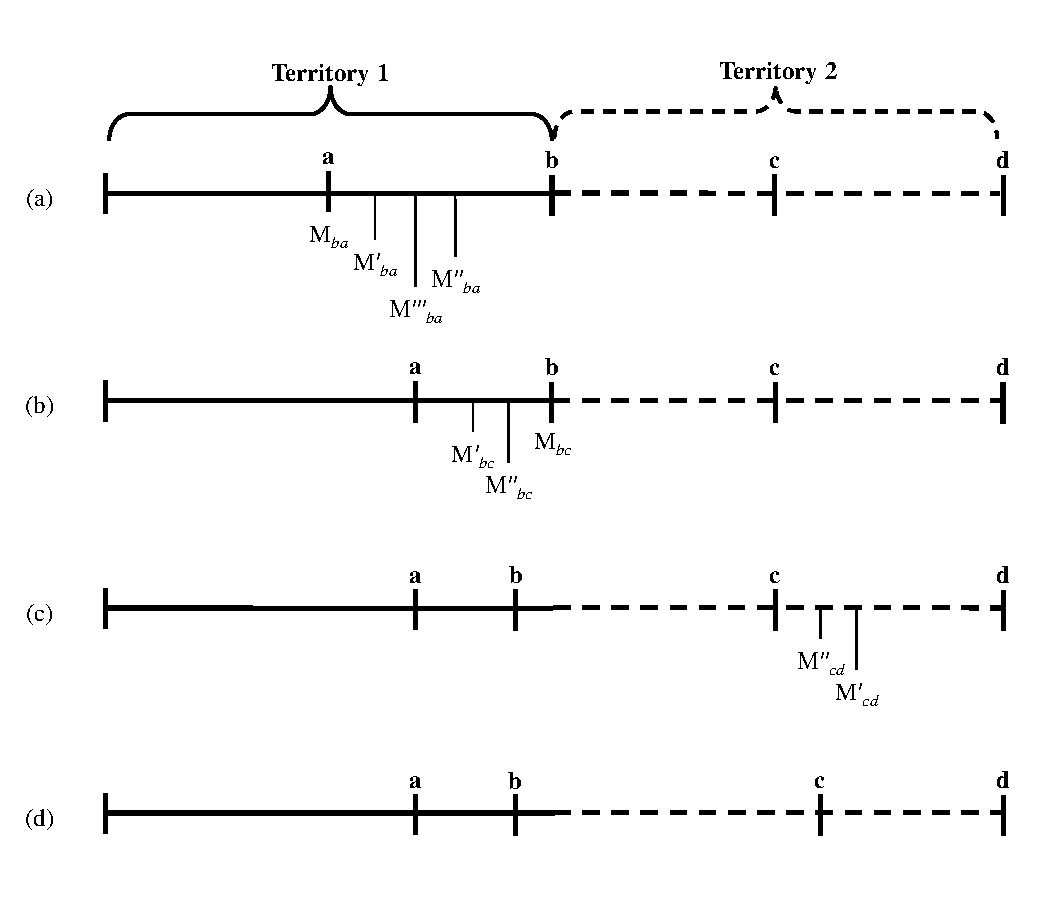
\includegraphics[scale=.92]{figures/territorial_competition.pdf}  
       \caption{Territorial competition between DTOs}
       \label{fig:territorial_competition}
\end{figure}


%%%%%%%%%%%%%%%%%%%%%%%%%%%%%%%%%%%%%%%%%%%%%%%%%%%%%%%%%%%%%%%%%%%%%%%%%%%%%%%%%%%%%%%%%%%%%%%%%%%%%







%%%%%%%%%%%%%%%%%%%%%%%%%%%%%%%%%%%%%%%%%%%%%%%%%%%%%%%%%%%%%%%%%%%%%%%%%%%%%%%%%%%%%%%%%%%%%%%%%%%%%

\newpage

\begin{figure}[h!]
      \centering
      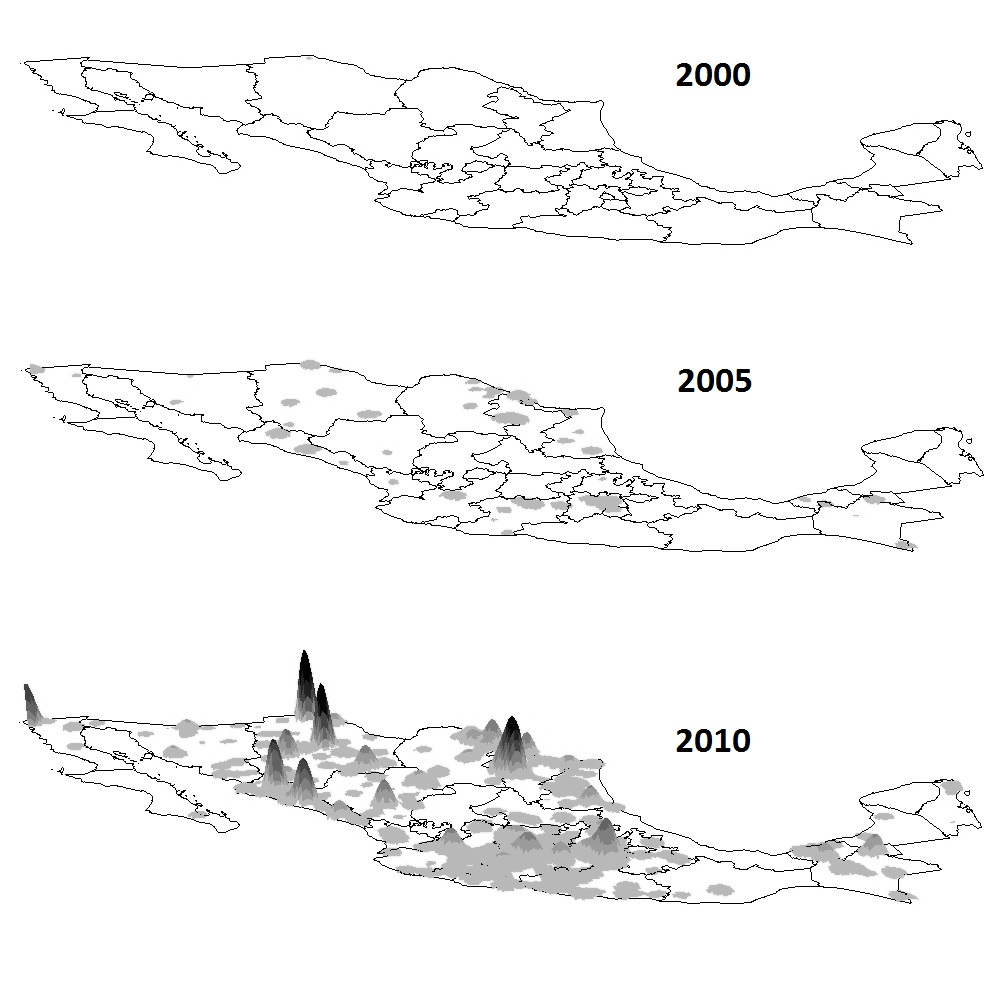
\includegraphics[scale=1.6]{figures/DVD_3D_00_05_10_BW.jpg}  
       \caption{Diffusion of violence between DTOs   \\(Cumulative Kernell density functions)}
       \label{fig:DVD_3D_2010}
\end{figure}


%%%%%%%%%%%%%%%%%%%%%%%%%%%%%%%%%%%%%%%%%%%%%%%%%%%%%%%%%%%%%%%%%%%%%%%%%%%%%%%%%%%%%%%%%%%%%%%%%%%%%

\newpage

\begin{figure}[h!]
      \centering
      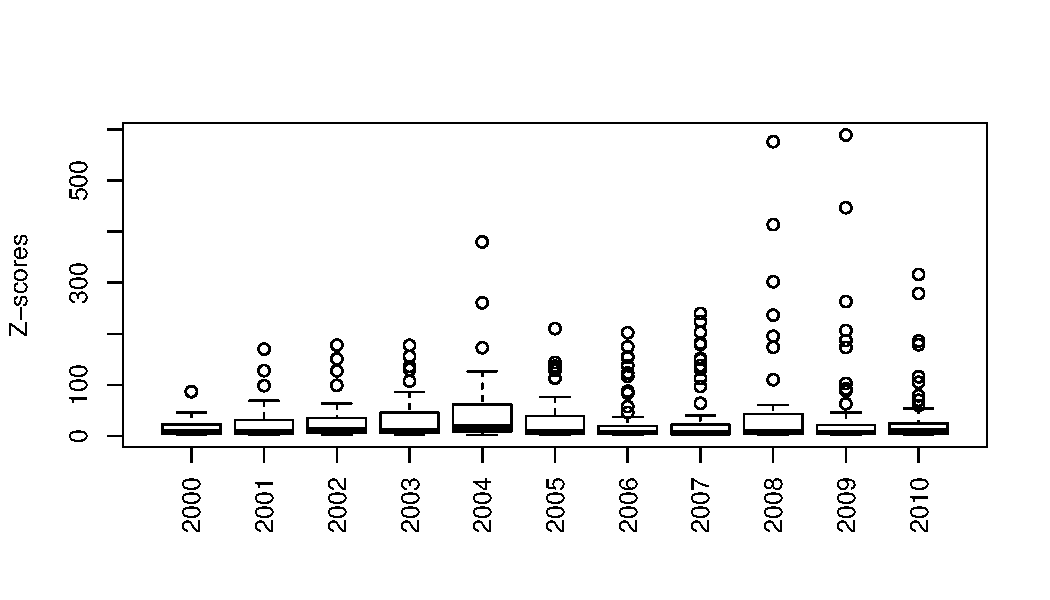
\includegraphics[scale=.9]{figures/local_outliers_box.pdf}  
       \caption{Outliers indicating the presence of local spatial autocorrelation}
       \label{fig:local_outliers_box}
\end{figure}



%%%%%%%%%%%%%%%%%%%%%%%%%%%%%%%%%%%%%%%%%%%%%%%%%%%%%%%%%%%%%%%%%%%%%%%%%%%%%%%%%%%%%%%%%%%%%%%%%%%%%



\newpage


\begin{landscape}

\begin{figure}[h!]
\centering
\subfigure[]{
    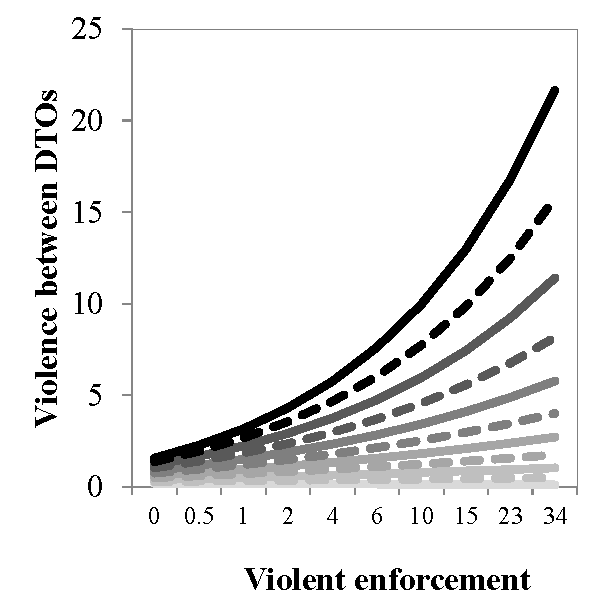
\includegraphics[width=.4\textwidth]{figures/mw1_SVD_NEW.pdf}
}
\subfigure[]{
    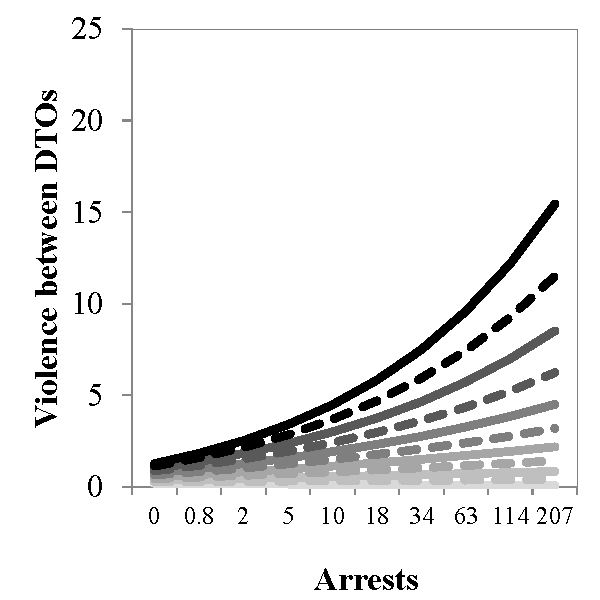
\includegraphics[width=.4\textwidth]{figures/mw1_SAD_NEW.pdf}
}
\subfigure[]{
    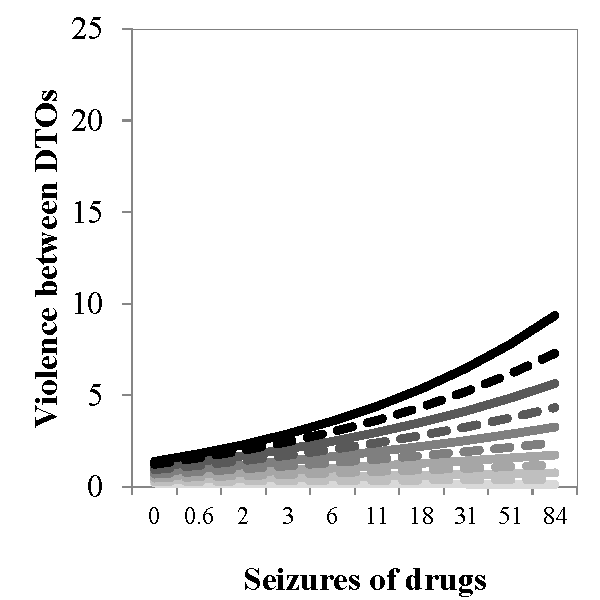
\includegraphics[width=.4\textwidth]{figures/mw1_SSD_NEW.pdf}
}
\subfigure[]{
    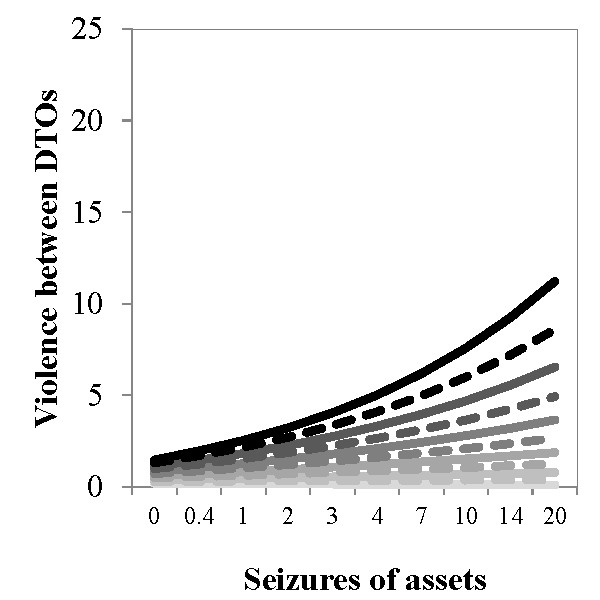
\includegraphics[width=.4\textwidth]{figures/mw1_SSA_NEW.pdf}
}
\subfigure[]{
    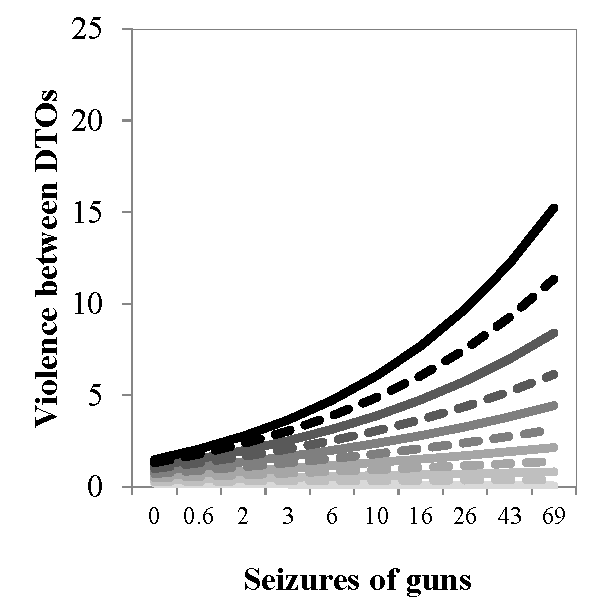
\includegraphics[width=.4\textwidth]{figures/mw1_SSG_NEW.pdf}
}
\subfigure[Legend]{
    \includegraphics[width=.4\textwidth]{figures/mw1_legend.pdf}
}
\caption{Predicted effects of violent and non-violent enforcement on violence among DTOs}
\label{fig:predicted_effects_allDTOS}
\end{figure}

\end{landscape}


%%%%%%%%%%%%%%%%%%%%%%%%%%%%%%%%%%%%%%%%%%%%%%%%%%%%%%%%%%%%%%%%%%%%%%%%%%%%%%%%%%%%%%%%%%%%%%%%%%%%%

\newpage

\begin{table}[h]
    \caption{Global Moran's I for violence between DTOs (2000--2010)}
    \label{tab:Global_Moran}
\begin{spacing}{0.85}
    \centering
    \begin{tabular}{ccccc}
    \hline
Year &  Observed I   &    Expected I &    Variance    &    p-value \\ \hline
2000 &    0.099    &    0.000    &    0.012    &    0.000 \\
2001 &    0.118	&	0.000	&	0.012	&	0.000 \\
2002 &	0.223	&	0.000	&	0.012	&	0.000 \\
2003 &	0.255	&	0.000	&	0.012	&	0.000 \\
2004 &	0.337	&	0.000	&	0.012	&	0.000 \\
2005 &	0.292	&	0.000	&	0.012	&	0.000 \\
2006 &	0.392	&	0.000	&	0.012	&	0.000 \\
2007 &	0.549	&	0.000	&	0.012	&	0.000 \\
2008 &	0.530	&	0.000	&	0.011	&	0.000 \\
2009 &	0.575	&	0.000	&	0.012	&	0.000 \\
2010 &	0.471	&	0.000	&	0.011	&	0.000 \\
\hline
\end{tabular}
\end{spacing}
\end{table}



%%%%%%%%%%%%%%%%%%%%%%%%%%%%%%%%%%%%%%%%%%%%%%%%%%%%%%%%%%%%%%%%%%%%%%%%%%%%%%%%%%%%%%%%%%%%%%%%%%%%%



\begin{landscape}

\begin{center}
\small
\begin{spacing}{0.85}
\begin{longtable}{lccccc}

\caption{Effect of law enforcement (lagged 4 weeks), all DTOs, and road density on violence between DTOs} \label{tab:enforcement_allDTOs_Road_L4L} \\

\hline 
\multicolumn{1}{l}{\textbf{Model }} &\multicolumn{1}{c}{\textbf{1}} & \multicolumn{1}{c}{\textbf{2}} & \multicolumn{1}{c}{\textbf{3}} & \multicolumn{1}{c}{\textbf{4}} & \multicolumn{1}{c}{\textbf{ 5}} \\ \hline 
\endfirsthead


\multicolumn{6}{c}{{\tablename\ \thetable{} -- continued from previous page}} \\ \hline
\multicolumn{1}{l}{\textbf{Model }} &\multicolumn{1}{c}{\textbf{1}} & \multicolumn{1}{c}{\textbf{2}} & \multicolumn{1}{c}{\textbf{3}} & \multicolumn{1}{c}{\textbf{4}} & \multicolumn{1}{c}{\textbf{ 5}} \\ \hline 
\endhead

\hline \multicolumn{6}{c}{{Continued on next page}} \\ \hline
\endfoot

\hline \hline
\endlastfoot

Lambda & 0.172*** & 0.172*** & 0.182*** & 0.175*** & 0.177***  \\ 
 & (0.004)  & (0.004)  & (0.004)  & (0.004)  & (0.004)   \\ 
                 
Violent enforcement (L4L) $\times$ All DTOs & 0.063*** &   &   &   &    \\ 
 & (0.001)  &   &   &   &    \\ 
Arrests  (L4L)  $\times$ All DTOs &   & 0.039*** &   &   &    \\ 
 &   & (0.000)  &   &   &    \\ 
Seizures of drugs  (L4L)  $\times$ All DTOs &   &   & 0.034*** &   &    \\ 
 &   &   & (0.000)  &   &    \\ 
 Seizures of assets  (L4L)  $\times$ All DTOs &   &   &   & 0.055*** &    \\ 
 &   &   &   & (0.000)  &    \\ 
 Seizures of guns  (L4L) $\times$ All DTOs &   &   &   &   & 0.047***  \\ 
 &   &   &   &   & (0.001)   \\ 
                 
Violent enforcement (L4L) $\times$ Road density & -49.222*** &   &   &   &    \\ 
 & (9.015)  &   &   &   &    \\ 
Arrests  (L4L)  $\times$ Road density &   & -12.226*** &   &   &    \\ 
 &   & (2.797)  &   &   &    \\ 
Seizures of drugs  (L4L)  $\times$ Road density &   &   & 20.278*** &   &    \\ 
 &   &   & (2.250)  &   &    \\ 
 Seizures of assets  (L4L)  $\times$ Road density &   &   &   & 2.587  &    \\ 
 &   &   &   & (5.050)  &    \\ 
 Seizures of guns  (L4L) $\times$ Road density &   &   &   &   & -85.494***  \\ 
 &   &   &   &   & (5.427)   \\ 
                 
Violent enforcement  (L4L)  & 0.008$^{\dag}$ &   &   &   &    \\ 
 & (0.004)  &   &   &   &    \\ 
Arrests  (L4L)  &   & -0.014*** &   &   &    \\ 
 &   & (0.001)  &   &   &    \\ 
Seizures of drugs  (L4L)  &   &   & -0.025*** &   &    \\ 
 &   &   & (0.001)  &   &    \\ 
Seizures of assets  (L4L)  &   &   &   & -0.031*** &    \\ 
 &   &   &   & (0.002)  &    \\ 
Seizures of guns  (L4L)  &   &   &   &   & 0.017***  \\ 
 &   &   &   &   & (0.002)   \\ 
                 
                 
                 
All DTOs & 0.077*** & 0.065*** & 0.069*** & 0.073*** & 0.073***  \\ 
 & (0.000)  & (0.000)  & (0.000)  & (0.000)  & (0.000)   \\ 
Road density & -3.844*** & -4.231*** & -4.092*** & -4.395*** & -4.214***  \\ 
 & (0.847)  & (1.031)  & (1.045)  & (0.935)  & (0.966)   \\ 
Drug production area & 0.000  & 0.000  & 0.000  & 0.000  & 0.000  \\ 
 & (0.000)  & (0.000)  & (0.000)  & (0.000)  & (0.000)   \\ 
Gulf & -0.004*** & -0.004** & -0.004** & -0.004*** & -0.004***  \\ 
 & (0.001)  & (0.001)  & (0.001)  & (0.001)  & (0.001)   \\ 
North & 0.017*** & 0.019*** & 0.019*** & 0.018*** & 0.017***  \\ 
 & (0.001)  & (0.002)  & (0.002)  & (0.002)  & (0.002)   \\ 
Pacific & 0.003** & 0.003* & 0.002* & 0.002$^{\dag}$ & 0.002*  \\ 
 & (0.001)  & (0.001)  & (0.001)  & (0.001)  & (0.001)   \\ 
Local drug market & 0.000** & 0.000*** & 0.000*** & 0.000*** & 0.000***  \\ 
 & (0.000)  & (0.000)  & (0.000)  & (0.000)  & (0.000)   \\ 
                 
Rifles & -0.003*** & -0.003*** & -0.003*** & -0.003*** & -0.003***  \\ 
 & (0.001)  & (0.001)  & (0.001)  & (0.001)  & (0.001)   \\ 
Potential cocaine production & 0.000*** & 0.000*** & 0.000*** & 0.000*** & 0.000***  \\ 
 & (0.000)  & (0.000)  & (0.000)  & (0.000)  & (0.000)   \\ 
Corruption & 0.000*** & 0.000*** & 0.000*** & 0.000*** & 0.000***  \\ 
 & (0.000)  & (0.000)  & (0.000)  & (0.000)  & (0.000)   \\ 
Schooling & 0.005*** & 0.006*** & 0.006*** & 0.006*** & 0.006***  \\ 
 & (0.000)  & (0.000)  & (0.000)  & (0.000)  & (0.000)   \\ 
Cocaine price & 0.000*** & 0.000*** & 0.000*** &  &   \\ 
 & (0.000)  & (0.000)  & (0.000)  &  &    \\ 
                 
Poverty & 0.009*** & 0.010*** & 0.010*** & 0.010*** & 0.010***  \\ 
 & (0.000)  & (0.000)  & (0.000)  & (0.000)  & (0.000)   \\ 
Population & 0.002*** & 0.002*** & 0.002*** & 0.002*** & 0.002***  \\ 
 & (0.000)  & (0.000)  & (0.000)  & (0.000)  & (0.000)   \\ 
Rate of violence among DTOs (lagged) & 0.011*** & 0.011*** & 0.011*** & 0.011*** & 0.011***  \\ 
 & (0.000)  & (0.000)  & (0.000)  & (0.000)  & (0.000)   \\ 
Constant & 0.007  & -0.003  & 0.004  & -0.010  & -0.003   \\ 
 & (0.012)  & (0.012)  & (0.012)  & (0.012)  & (0.012)   \\ \hline
                 
Rho & -0.117  & -0.108  & -0.120  & -0.117  & -0.120   \\ 
% Sigma$^{2}V$ & 0.012  & 0.012  & 0.012  & 0.012  & 0.012   \\ 
% Sigma$^{2}V$ & 0.169  & 0.255  & 0.264  & 0.210  & 0.225   \\ 
% Theta & 0.733  & 0.783  & 0.786  & 0.760  & 0.769   \\ 
                 
Observations  &  1,657,800   &  1,657,800   &  1,657,800   &  1,657,800   &  1,657,800    \\ \hline

\multicolumn{6}{l}{``L4L'' refers to event data lagged four weeks and logged.  *** p< 0.001, ** p< 0.01, * p< 0.05, $^{\dag}$ p< 0.1} \\
%\multicolumn{6}{l}{} \\

\end{longtable}
\end{spacing}
\end{center}
%\end{landscape}


%%%%%%%%%%%%%%%%%%%%%%%%%%%%%%%%%%%%%%%%%%%%%%%%%%%%%%%%%%%%%%%%%%%%%%%%%%%%%%%%%%%%%%%%%%%%%%%%%%%%%




%%%%%%%%%%%%%%%%%%%%%%%%%%%%%%%%%%%%%%%%%%%%%%%%%%%%%%%%%%%%%%%%%%%%%%%%%%%%%%%%%%%%%%%%%%%%%%%%%%%%%



%\begin{landscape}
\begin{center}
\small
\begin{spacing}{0.85}
\begin{longtable}{lccccc}

\caption{Effect of law enforcement (lagged 4 weeks), main and secondary DTOs, and road density on violence between DTOs} \label{tab:enforcement_MainMinorDTOs_Road_L4L} \\

\hline 
\multicolumn{1}{l}{\textbf{Model }} &\multicolumn{1}{c}{\textbf{6}} & \multicolumn{1}{c}{\textbf{7}} & \multicolumn{1}{c}{\textbf{8}} & \multicolumn{1}{c}{\textbf{9}} & \multicolumn{1}{c}{\textbf{10}} \\ \hline 
\endfirsthead


\multicolumn{6}{c}{{\tablename\ \thetable{} -- continued from previous page}} \\ \hline
\multicolumn{1}{l}{\textbf{Model }} &\multicolumn{1}{c}{\textbf{6}} & \multicolumn{1}{c}{\textbf{7}} & \multicolumn{1}{c}{\textbf{8}} & \multicolumn{1}{c}{\textbf{9}} & \multicolumn{1}{c}{\textbf{10}} \\ \hline 
\endhead

\hline \multicolumn{6}{c}{{Continued on next page}} \\ \hline
\endfoot

\hline \hline
\endlastfoot

Lambda & 0.167*** & 0.169*** & 0.177*** & 0.171*** & 0.172*** \\ 
 & (0.004) & (0.004) & (0.004) & (0.004) & (0.004) \\ 
Violent enforcement (L4L) $\times$ Main DTOs & 0.096*** & & & & \\ 
 & (0.001) & & & & \\ 
Arrests (L4L) $\times$ Main DTOs & & 0.041*** & & & \\ 
 & & (0.000) & & & \\ 
Seizures of drugs (L4L) $\times$ Main DTOs & & & 0.033*** & & \\ 
 & & & (0.000) & & \\ 
Seizures of assets (L4L) $\times$ Main DTOs & & & & 0.057*** & \\ 
 & & & & (0.001) & \\ 
Seizures of guns (L4L) $\times$ Main DTOs & & & & & 0.054*** \\ 
 & & & & & (0.001) \\ 
 
Violent enforcement (L4L) $\times$ Secondary DTOs & -0.048*** & & & & \\ 
 & (0.002) & & & & \\ 
Arrests (L4L) $\times$ Secondary DTOs & & 0.017*** & & & \\ 
 & & (0.001) & & & \\ 
Seizures of drugs (L4L) $\times$ Secondary DTOs & & & 0.028*** & & \\ 
 & & & (0.001) & & \\ 
Seizures of assets (L4L) $\times$ Secondary DTOs & & & & 0.033*** & \\ 
 & & & & (0.002) & \\ 
Seizures of guns (L4L) $\times$ Secondary DTOs & & & & & 0.007*** \\ 
 & & & & & (0.002) \\ 
 
Violent enforcement (L4L) $\times$ Road density & -45.224*** & & & & \\ 
 & (9.006) & & & & \\ 
Arrests (L4L) $\times$ Road density & & -13.290*** & & & \\ 
 & & (2.799) & & & \\ 
Seizures of drugs (L4L) $\times$ Road density & & & 18.239*** & & \\ 
 & & & (2.251) & & \\ 
Seizures of assets (L4L) $\times$ Road density & & & & 1.425 & \\ 
 & & & & (5.049) & \\ 
Seizures of guns (L4L) $\times$ Road density & & & & & -86.003*** \\ 
 & & & & & (5.430) \\ 
 
Violent enforcement (L4L) & -0.021*** & & & & \\ 
 & (0.004) & & & & \\ 
Arrests (L4L) & & -0.013*** & & & \\ 
 & & (0.001) & & & \\ 
Seizures of drugs (L4L) & & & -0.022*** & & \\ 
 & & & (0.001) & & \\ 
Seizures of assets (L4L) & & & & -0.028*** & \\ 
 & & & & (0.002) & \\ 
Seizures of guns (L4L) & & & & & 0.016*** \\ 
 & & & & & (0.002) \\ 
 
Main DTOs & 0.067*** & 0.058*** & 0.061*** & 0.065*** & 0.064*** \\ 
 & (0.000) & (0.000) & (0.000) & (0.000) & (0.000) \\ 
Minor DTOs & 0.129*** & 0.109*** & 0.113*** & 0.117*** & 0.123*** \\ 
 & (0.001) & (0.001) & (0.001) & (0.001) & (0.001) \\ 
Road density & -3.374*** & -3.459*** & -3.400** & -3.414*** & -3.223*** \\ 
 & (0.826) & (1.015) & (1.036) & (0.933) & (0.939) \\ 
 
Drug production area & 0.000 & 0.000$^{\dag}$ & 0.000* & 0.000$^{\dag}$ & 0.000 \\ 
 & (0.000) & (0.000) & (0.000) & (0.000) & (0.000) \\ 
Gulf & -0.005*** & -0.004*** & -0.004*** & -0.004*** & -0.005*** \\ 
 & (0.001) & (0.001) & (0.001) & (0.001) & (0.001) \\ 
North & 0.018*** & 0.019*** & 0.019*** & 0.019*** & 0.018*** \\ 
 & (0.001) & (0.002) & (0.002) & (0.002) & (0.002) \\ 
Pacific & 0.003** & 0.003* & 0.003* & 0.002* & 0.003* \\ 
 & (0.001) & (0.001) & (0.001) & (0.001) & (0.001) \\ 
Poverty & 0.008*** & 0.010*** & 0.010*** & 0.009*** & 0.009*** \\ 
 & (0.000) & (0.000) & (0.000) & (0.000) & (0.000) \\ 
Population & 0.002*** & 0.003*** & 0.003*** & 0.002*** & 0.002*** \\ 
 & (0.000) & (0.000) & (0.000) & (0.000) & (0.000) \\ 
Rifles & 0.001 & 0.001 & 0.000 & 0.000 & 0.000 \\ 
 & (0.001) & (0.001) & (0.001) & (0.001) & (0.001) \\ 
Potential cocaine production & 0.000*** & 0.000*** & 0.000*** & 0.000*** & 0.000*** \\ 
 & (0.000) & (0.000) & (0.000) & (0.000) & (0.000) \\ 
Schooling & 0.005*** & 0.006*** & 0.006*** & 0.006*** & 0.006*** \\ 
 & (0.000) & (0.000) & (0.000) & (0.000) & (0.000) \\ 
Rate of violence among DTOs (lagged) & 0.011*** & 0.011*** & 0.011*** & 0.011*** & 0.011*** \\ 
 & (0.000) & (0.000) & (0.000) & (0.000) & (0.000) \\ 
Constant & -0.055*** & -0.061*** & -0.056*** & -0.054*** & -0.048*** \\ 
 & (0.012) & (0.012) & (0.012) & (0.012) & (0.012) \\ \hline
 
Rho & -0.0747 & -0.0722 & -0.0759 & -0.0747 & -0.0769 \\ 
% Sigma$^{2}V$ & 0.0117 & 0.0117 & 0.0117 & 0.0117 & 0.0117 \\ 
% Sigma$^{2}V$ & 0.0001 & 0.0001 & 0.0001 & 0.0001 & 0.0001 \\ 
% Theta & -11.8120 & -11.8660 & -11.8340 & -11.8410 & -11.8870 \\ 
 
Observations & 1,657,800 & 1,657,800 & 1,657,800 & 1,657,800 & 1,657,800 \\ \hline


\hline  
\multicolumn{6}{l}{``L4L'' refers to event data lagged four weeks and logged.  *** p< 0.001, ** p< 0.01, * p< 0.05, $^{\dag}$ p< 0.1} \\
%\multicolumn{6}{l}{} \\
 

\end{longtable}
\end{spacing}
\end{center}
\end{landscape}



%%%%%%%%%%%%%%%%%%%%%%%%%%%%%%%%%%%%%%%%%%%%%%
%%%%%%%%%%%%%%%%%%%%%%%%%%%%%%%%%%%%%%%%%%%%%%
%%
%% APPENDIX HERE
%%
%%%%%%%%%%%%%%%%%%%%%%%%%%%%%%%%%%%%%%%%%%%%%%
%%%%%%%%%%%%%%%%%%%%%%%%%%%%%%%%%%%%%%%%%%%%%%





\end{document}
